\section{Описание инструмента}

Целью данной работы является создание инструмента для автоматического обнаружения архитектурных антипаттернов и других нарушений заданных принципов в микросервисных системах. Основная задача инструмента — предоставить архитекторам и разработчикам удобное и гибкое средство для контроля за состоянием архитектуры и количественной оценки технического долга. Инструмент позволяет описывать правила любой сложности и органично интегрируется с существующей инфраструктурой Яндекс.Вертикалей. В данном разделе будет подробно описано его устройство, а также предоставляемое пользователям API.

\subsection{Верхнеуровневая архитектура}

\begin{figure}[ht]
    \centering
    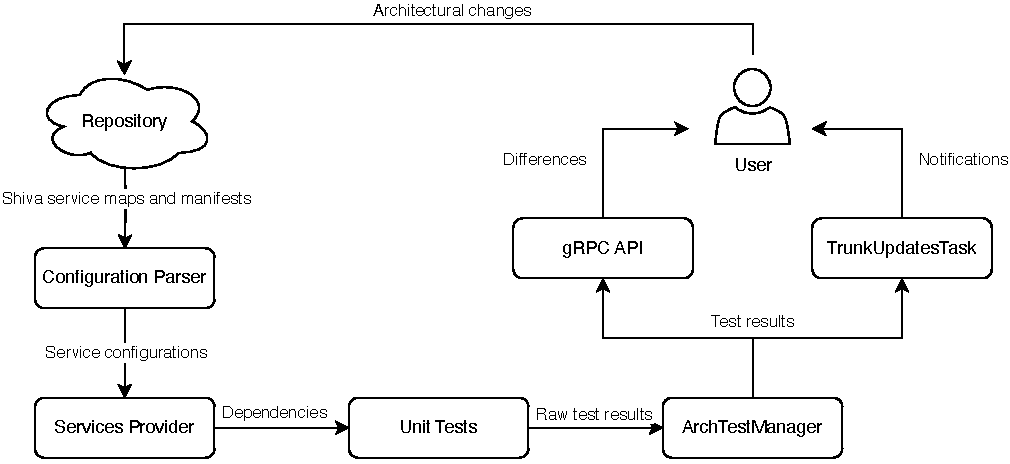
\includegraphics[scale=0.9]{images/archtest-components.drawio.pdf}
    \caption{\label{archtest-components} Ключевые компоненты и их взаимодействие.}
\end{figure}

Основные компоненты приложения, а также их взаимодействие между собой и с пользователем представлено на рисунке \ref{archtest-components}. Таким образом, приложение состоит из нескольких модулей:

\begin{itemize}
    \item \textbf{Модуль загрузки и парсинга конфигураций}. Отвечает за получение данных об архитектуре анализируемой системы.
    \item \textbf{Архитектурные правила}. Могут быть заданы двумя способами: в виде unit-тестов на языке Scala или декларативно в формате YAML.
    \item \textbf{Модуль выполнения тестов}. Управляет процессом запуска архитектурных проверок и выставляет программное API для получения агрегированных результатов прогона тестов.
    \item \textbf{gRPC API} \cite{grpc-fw}. Предоставляет удобные методы для интеграции инструмента с CI/CD и автоматической проверки изменений в пулл-реквестах.
    \item \textbf{TrunkUpdatesTask}. Отслеживает изменения в основной ветке разработки (trunk \cite{trunk-based-dev}) и отправляет уведомления в Telegram при обнаружении новых архитектурных проблем.
\end{itemize}

В следующих разделах будет подробно рассмотрен каждый из перечисленных компонентов.

\subsection{Загрузка и парсинг конфигураций}

Источником данных для тестов служат конфигурационные файлы системы развертывания Shiva: карты сервисов и манифесты деплоя. Инструмент умеет получать эти файлы либо из системы контроля версий Arcadia \cite{arcadia} для указанной ревизии (коммита или ветки), либо из локальной файловой системы. Это позволяет анализировать как любой заданный срез архитектуры в прошлом, так и текущее локальное состояние. Загруженные YAML-файлы проходят через стадию парсинга и преобразуются во внутреннюю модель системы. Эта модель представляет собой граф, узлами которого являются сущности типа \verb|Service|, а рёбрами — зависимости между ними. Каждый объект \verb|Service| содержит информацию об имени сервиса, его типе, предоставляемых интерфейсах и зависимостях: как явных, указанных в \verb|depends_on|, так и неявных, содержащихся в переменных окружения из конфигурации. Помимо этих полей в \verb|Service| содержится и другая метаинформация о сервисе, которую предоставляет Shiva.

\subsection{Написание unit-тестов}\label{unit-tests-design}

Основным и наиболее гибким способом описания архитектурных правил является создание unit-тестов на языке Scala с использованием фреймворка ScalaTest \cite{scalatest-fw}. Для этого разработчикам предоставляется специальный трейт \verb|ArchTest|, который необходимо унаследовать в классе с тестами. Этот трейт обеспечивает доступ к загруженной и обработанной модели архитектуры, а также предоставляет вспомогательные методы для написания проверок. Как уже упоминалось, при локальном запуске тестов будет использована текущая локальная конфигурация сервисов Shiva.

Вместо построения явного графа зависимостей, здесь используется несколько другой подход: \verb|ArchTest| предоставляет список всех сервисов \verb|services: Seq[Service]|, внутри каждого из которых содержится вся информация о его зависимостях. Чтобы проверить наличие зависимости между сервисами \verb|A| и \verb|B|, нужно вызвать метод \verb|hasDependencyOn| у \verb|A|. Метод просканирует секцию \verb|depends_on| и все переменные окружения сервиса \verb|A| на упоминание сервиса \verb|B|. Если оно будет найдено, то метод возвращает \verb|true|. Более формально это отражено в алгоритме \ref{has-dependency-on}.

\begin{algorithm}[hbt!]
\caption{Проверка зависимости от другого сервиса}\label{has-dependency-on}

\SetKwProg{hasDependencyOn}{hasDependencyOn}{}{}
\hasDependencyOn{$(this, other)$}{
\KwData{$this$ — текущий сервис со своими зависимостями}
\KwData{$other$ — другой сервис для проверки}

$inDependsOn \gets \text{false}$\;
\ForEach{$dependency \in this.dependsOn$}{
    \If{$\text{matches}(other, dependency)$}{
        $inDependsOn \gets \text{true}$\;
        \textbf{break}\;
    }
}

$inConfig \gets \text{false}$\;
\ForEach{$envVariable \in this.config.envVariables$}{
    \If{$\text{matches}(other, envVariable)$}{
        $inConfig \gets \text{true}$\;
        \textbf{break}\;
    }
}

\Return $inDependsOn \lor inConfig$\;
}
\end{algorithm}

Алгоритм использует функцию \verb|matches|, чтобы проверить совпадение сервиса \verb|other| с очередным сервисом из \verb|depends_on| или с очередной переменной окружения \verb|envVariable|. Подробнее про внутреннее устройство этой функции будет написано в одном из следующих разделов, а пока что можно воспринимать её работу <<естественно>>: сервисы могут совпасть по имени, по URL и так далее.

Помимо основного \verb|hasDependencyOn|, библиотека предоставляет другие полезные функции для разных сценариев использования:

\begin{itemize}
    \item \verb|hasDependencyInServiceMap|: Проверяет только явные зависимости из \verb|depends_on|.
    \item \verb|hasDependencyInConfig|: Проверяет только зависимости, выведенные из переменных окружения (например, URL другого сервиса или строки подключения к БД).
    \item \verb|hasDependencyOn(other: ServicePattern)|: Работает аналогично основному методу, но принимает не существующий в системе \verb|Service|, а описанный пользователем \verb|ServicePattern|. Паттерн позволяет гибко задавать критерии поиска целевого сервиса (по имени, типу, хосту, IP-адресу и так далее).
\end{itemize}

Для иллюстрации рассмотрим простой пример теста, который проверяет, что сервис \verb|payment-service| не должен напрямую зависеть от базы данных пользователей \verb|user-db| (допустим, что такие компоненты есть в нашей системе).

\begin{code}{scala}
"payment-service" should "not access user-db" in {
  val paymentService = Services.service("payment-service")
  val userDb = Services.mysql("user-db")

  paymentService.hasDependencyOn(userDb) shouldBe false
}
\end{code}

\verb|Services.service("payment-service")| является удобным способом получить экземпляр \verb|Service| для сервиса с именем "payment-service". Для базы данных \verb|user-db| используется аналогичный метод \verb|Services.mysql|.

Другой пример: проверка, что только \verb|orders-proxy| может зависеть от внешней системы \verb|orders.com|.

\begin{code}{scala}
"orders.com" should "only be accessed by orders-proxy" in {
  val ordersProxy = Services.service("orders-proxy")
  val ordersCom = ServicePattern.withHost("orders.com")

  val ordersComDependents = services.filter { service =>
    service.hasDependencyOn(ordersCom)
  }

  ordersComDependents shouldBe Seq(ordersProxy)
}
\end{code}

Здесь мы итерируемся по всем сервисам и проверяем условие, что только прокси имееет прямую зависимость на внешнюю систему.

\subsection{Задание проверок в YAML-конфиге}

Для простых и типовых архитектурных правил инструмент позволяет описывать их в декларативном стиле с помощью YAML-файлов \cite{yaml-spec}. Это может быть удобно для для быстрого добавления стандартных проверок без написания Scala-кода.

Каждый YAML-файл может содержать список правил. Структура правила определяется следующими полями:
\begin{itemize}
    \item \verb|rule|: Человекочитаемое описание правила.
    \item \verb|service|: Определяет сервис или группу сервисов, к которым применяется правило. Содержит обязательное поле \verb|name|, значение которого интерпретируется как регулярное выражение для полного имени сервиса (например, \verb|mysql/user-db| или \verb|payment-service|). Структура задумывалась расширяемой, чтобы в дальнейшем можно было задавать сервис не только по имени, а, например, по владельцу или другой метаинформации.
    \item \verb|dependencies| (опционально): Определяет ограничения на исходящие зависимости проверяемого сервиса. Может содержать либо \verb|whitelist| (список разрешенных сервисов-зависимостей), либо \verb|blacklist| (список запрещенных сервисов-зависимостей). Элементы в \verb|whitelist| и \verb|blacklist| являются <<сервисами>>, то есть могут быть также заданы по имени с помощью регулярного выражения.
    \item \verb|dependents| (опционально): Определяет ограничения на входящие зависимости (сервисы, которые зависят от проверяемого сервиса). Структура аналогична \verb|dependencies|.
\end{itemize}

Важно, что в рамках одного блока (\verb|dependencies| или \verb|dependents|) нельзя одновременно использовать \verb|whitelist| и \verb|blacklist|, так как это не имеет смысла.

Для иллюстрации возможностей правил в YAML, перепишем unit-тест про \verb|payment-service| из предыдущего раздела декларативно.

\begin{nocode}
- rule: "payment-service should not access user-db"
  service:
    name: mysql/user-db
  dependents:
    blacklist:
      - name: payment-service
\end{nocode}

Другой пример: сервисы catalog-api и catalog-tasks не должны ни от кого зависеть.

\begin{nocode}
- rule: "catalog should not depend on other services"
  service:
    name: catalog-(api|tasks)
  dependencies:
    whitelist: []
\end{nocode}

Разбор и выполнение таких YAML-правил осуществляется специальным ScalaTest-тестом \verb|YamlSpec|. Он находит все \verb|*.yml| файлы в заданной директории, парсит их и для каждого правила из файла динамически генерирует соответствующие проверки во время выполнения тестов.

\subsection{Запуск тестов в рантайме}

Библиотека для написания архитектурных тестов разработана таким образом, чтобы их можно было запускать не только локально из IDE, но и программно, например, по запросу или периодически. Эту функциональность обеспечивает \verb|ArchTestManager|. Когда \verb|ArchTestManager| получает запрос на запуск тестов для определённой ревизии (коммита или имени ветки), ему необходимо каким-то образом передать в тесты нужную версию инфраструктурных схем. Для этого он устанавливает системное свойство JVM \verb|archtest.run_mode|. Значением этого свойства является JSON-строка, представляющая объект \verb|RunMode|, например,

\begin{zerocode}{json}
{
    "mode": "Branch",
    "revision": "my-feature-branch",
    "arc_config": {
        "token": "<ARC_TOKEN>",
        "path": "/opt/homebrew/bin/arc"
    }
}
\end{zerocode}

Использование \verb|System.setProperty| для передачи параметров запуска является ключевым моментом. Стандартный механизм \verb|ConfigMap| из ScalaTest здесь не подходит, поскольку он становится доступен уже после обнаружения и инициализации тестовых классов. В нашем же случае, конфигурация (режим запуска, ревизия) нужна на самом раннем этапе – до того, как ScalaTest начнет исполнять тесты, и даже до того как он полностью определит их список. Это связано с тем, что сама структура архитектуры (и, как следствие, набор сервисов, для которых могут генерироваться тесты) зависит от выбранной ревизии.

После установки системного свойства, \verb|ArchTestManager| запускает стандартный \verb|scalatest.Runner|. Он обнаруживает все скомпилированные тестовые классы, и при инстанцировании каждого такого класса, благодаря подмешанному трейту \verb|ArchTest|, происходит следующее:

\begin{enumerate}
    \item Читается системное свойство \verb|archtest.run_mode|.
    \item На основе этого свойства выбирается и конфигурируется соответствующий провайдер данных (например, \verb|ServicesProviderArcadia| для режима \verb|Branch|).
    \item Выбранный провайдер загружает конфигурационные файлы Shiva для заданной ревизии (из Arcadia или локально).
    \item Загруженные файлы парсятся, и строится полная внутренняя модель системы в виде последовательности объектов \verb|Seq[Service]|.
    \item Эта модель становится доступной внутри тестового класса через поле \verb|lazy val services: Seq[Service]|, и уже на ее основе выполняются проверки.
\end{enumerate}

Результаты выполнения тестов (успех/неудача, сообщения об ошибках и т.д.) собираются с помощью кастомной реализации \verb|scalatest.Reporter|. Он подписывается на события \verb|TestSucceeded| и \verb|TestFailed|, которые генерирует ScalaTest во время выполнения тестов, и собирает информацию о результатах прогона. В итоге они возвращаются в виде структурированных объектов \verb|RunTestResult| в вызывающий код.

\subsection{Валидация изменений в пулл реквесте}

Одна из основных задач инструмента — предотвращение попадания нежелательных архитектурных изменений в основную ветку разработки (trunk). Для этого инструмент предоставляет возможность сравнить результаты архитектурных тестов между текущей веткой разработки (например, веткой пулл-реквеста) и её точкой расхождения с trunk, так называемой merge-base. Эта логика реализована в \verb|ArchTestManager| и доступна через gRPC-метод \verb|compareTestsWithTrunk|.

При вызове этого метода с указанием имени проверяемой ветки, gRPC-сервис определяет merge-base и дважды запускает архитектурные тесты: для указанной ветки и для merge-base. После этого результаты двух запусков сравниваются, и выделяются различия: новые упавшие тесты (потенциальные проблемы), исправленные тесты (улучшения), а также добавленные или удаленные тесты. Эта информация возвращается через gRPC и может быть использована CI/CD системой для автоматического комментирования пулл-реквеста, информируя разработчиков и ревьюеров о влиянии предлагаемых изменений на архитектуру.

На данный момент, непосредственная интеграция с интерфейсом систем управления версиями (в случая Яндекса — это Arcanum) для публикации комментариев в пулл-реквестах не реализована, так как было принято решение сначала провести апробацию инструмента и оценку его эффективности в более узком кругу разработчиков. Однако весь необходимый функционал на стороне бэкенда для такой интеграции уже существует и запущен в облаке.

\subsection{Уведомления в Telegram}

В качестве основного способа обратной связи на текущем этапе и для поэтапного внедрения инструмента была выбрана система уведомлений об архитектурных изменениях в основной ветке (trunk) через Telegram. Это решение является временной альтернативой полноценной интеграции проверок в процесс код-ревью, позволяя избежать немедленной раскатки новой функциональности на всех разработчиков компании (которые неизбежно столкнулись бы с инструментом при работе с пулл-реквестами). Такой подход даёт возможность узкому кругу заинтересованных лиц апробировать инструмент, собрать обратную связь и оценить его пользу в реальных условиях без широкого анонсирования. Реализацию этого непрерывного мониторинга обеспечивает фоновая задача \verb|TrunkUpdatesTask|. Важно отметить, что даже после полного запуска валидации в пулл-реквестах, \verb|TrunkUpdatesTask| сохранит свою актуальность: она будет служить дополнительным уровнем контроля для архитекторов, информируя их о случаях, когда архитектурные нарушения все же могли быть пропущены или сознательно внесены в основную ветку разработки.

\verb|TrunkUpdatesTask| с настраиваемой периодичностью запрашивает историю коммитов в репозиторий с инфраструктурными схемами Shiva. Для каждой пары последовательных коммитов (старый и новый) запускается сравнение результатов архитектурных тестов. Если обнаруживаются различия (например, тест, который проходил в старом коммите, начал падать в новом, или наоборот), формируется соответствующее уведомление в Telegram.

Ключевую роль в системе уведомлений играет механизм тегирования результатов тестов и конфигурация подписок.
Система уведомлений может понимать контекст упавшего или исправленного теста и отправлять сообщение только тем, кому данный тест может быть интересен. Для этого все тесты снабжаются тегами с помощью метода \verb|report|. Предусмотрено несколько способов вызова:
\begin{itemize}
    \item \verb|report(service: Service*)|: Автоматически добавляет стандартный набор тегов для указанных сервисов: их полное имя, владельцев и некоторые другие поля. Например, \verb|report(myService)| добавит тег \verb|"fqn": "my-service"|, \verb|"owner": "..."| и так далее. Более того, для удобства написания тестов сделано так, что обращение к функции \verb|Services.service| само по себе вызывает \verb|report| на переданном сервисе.
    \item \verb|report(key: String, value: String)|: Добавляет пользовательский тег, например, \verb|report("tag", "critical")|.
\end{itemize}

Технически, метод \verb|report| вызывает \verb|note| из ScalaTest, передавая строку с тегами в специальном формате. Уже упомянутый ранее кастомный \verb|scalatest.Reporter| перехватывает события \verb|NoteProvided| и извлекает теги, прикрепляя их к результату соответствующего теста (\verb|RunTestResult|).

Сформированные уведомления и ассоциированные с ними теги передаются в \verb|TelegramNotifier|. Последний, на основе конфигурации подписок, определяет, каким пользователям или в какие чаты следует отправить сообщение. Конфигурация подписок загружается в рантайме из системы управления фича-флагами и представляет собой YAML-структуру следующего вида:

\begin{itemize}
    \item \verb|name|: Человекочитаемое описание подписки.
    \item \verb|enabled|: Включена ли данная подписка или нет.
    \item \verb|chat_ids|: Список числовых ID чатов Telegram, куда нужно отправлять уведомления по данной подписке.
    \item \verb|conditions|: Список условий для срабатывания подписки. Сообщение будет отправлено, если результат теста удовлетворяет всем условиям из этого списка (логическое "И"). Каждое условие — это пара, где ключ — это имя тега (например, \verb|fqn|, \verb|owner|, \verb|tag| и т.д.), а значение — список допустимых строковых значений. Для того чтобы условие по ключу считалось выполненным, тег с таким ключом у результата теста должен иметь хотя бы одно из значений, перечисленных в списке (логическое "ИЛИ"). Например, условие \verb|fqn: ["service-a", "service-b"]| сработает, если имя сервиса, связанного с тестом, равняется \verb|service-a| или \verb|service-b|.
\end{itemize}

Ниже приведен пример с двумя подписками на уведомления.

\begin{nocode}
subscriptions:
  - name: "Critical issues for Team A"
    enabled: true
    chat_ids:
      - 123456789
      - 987654321
    conditions:
      - tag: ["critical"] 
      - owner: ["team-a"]
  - name: "All payment service issues"
    enabled: true
    chat_ids:
      - 112233445 
    conditions:
      - fqn: ["payment-api", "payment-tasks"]
\end{nocode}

Пример уведомления в Telegram показан на рисунке \ref{telegram-notification-example}.
